\documentclass{beamer}

\usepackage[UTF8,noindent]{ctexcap}
\usepackage{color}%引入颜色
\usetheme{Berlin}%使用Singapore主题
\usepackage{graphicx}%引入插图
\usepackage{ulem}%删除线
\usepackage{tikz}
\usefonttheme[onlymath]{serif}
\usepackage{minted}%[fragile]
\useoutertheme{infolines}
%\usepackage[orientation=landscape,size=custom,width=16,height=9,scale=0.5,debug]{beamerposter}

\title{图论+树上问题 杂题选讲}
\date{2021年8月21日}
\author{租酥雨}
\begin{document}\small
	
	%\usebackgroundtemplate{\tikz\node[inner sep=0pt,opacity=0.3]{\includegraphics[width=16cm,height=9cm]{zsy_background.jpg}};}
	\begin{frame}
		\titlepage
		\begin{center}
			
\includegraphics[width=2.0cm]{zsy.jpg}
		\end{center}
	\end{frame}


\subsection{PA2014 Kuglarz}
\begin{frame}{PA2014 Kuglarz}
	\begin{block}{description}
		$n$个倒置的杯子排成一行,有些杯子底下藏着一个小球,另一些没藏。
		
		你可以花费$c_{ij}$的代价询问杯子$i, i+1, \cdots, j$底下藏着的球的数量的奇偶性。
		
		求根据询问信息猜出每个杯子底下有没有藏球所需的最小总代价。
	\end{block}
	\begin{block}{constraint}
		$n \le 5000.$
	\end{block}
\end{frame}
\begin{frame}{PA2014 Kuglarz}
	\begin{block}{tutorial}
		转化为前缀和,每次询问相当于是得到了某两个前缀和之间的相等关系。\\
		
		已知$s_0 = 0$,需要通过相等关系让$s_1, \cdots, s_n$与$s_0$“连通”,那么求一棵最小生成树即可。
	\end{block}
\end{frame}

\subsection{Lydsy1705月赛 棋盘上的守卫}
\begin{frame}{Lydsy1705月赛 棋盘上的守卫}
	\begin{block}{description}
		有一张$n \times m$的棋盘,你需要选择一些位置放置守卫。守卫分为两种:横向守卫与纵向守卫。
		
		每个位置放置守卫的代价是不同的,但同一个位置上方式横向或纵向守卫的代价是相同的。
		
		求为了满足“每行有至少一个横向守卫,每列有至少一个纵向守卫”的要求,所需的最小代价。
	\end{block}
	\begin{block}{constraint}
		$n \times m \le 10^6$,所有代价均非负。
	\end{block}
\end{frame}
\begin{frame}{Lydsy1705月赛 棋盘上的守卫}
	\begin{block}{tutorial}
		对每行每列分别建立一个点,记第$i$行对应的点是$a_i$,第$j$列对应的点是$b_j$,对于一个$(x, y)$处的守卫,若它是横向的,则连边$a_x \to b_y$,否则连边$b_y \to a_x$。\\
		
		这样转化后,问题的限制等价于对于这$n + m$个点,需要选取一些边使每个点的出度都恰好为$1$。\\
		
		会发现只需要让每个连通块构成一棵基环树,就一定存在一种给边定向(给守卫确定横纵向)的方案使这个连通块满足限制。\\
		
		所以只需要对这张图求“最小生成基环树森林”就可以了。
	\end{block}
\end{frame}


\subsection{例题:tree}
\begin{frame}{例题:tree}
	\begin{block}{description}
		一张$n$个点$m$条边的带权无向图,边有黑白两色。求恰好有$k$条白边的边权和最小的生成树。
	\end{block}
	\begin{block}{constraint}
		$n, m \le 10^5.$
	\end{block}
\end{frame}
\begin{frame}{例题:tree}
	\begin{block}{tutorial}
		给每条白边加上一个权值偏置$Bias$,直接做最小生成树,那么生成树中白边的数量关于$Bias$是单调的(需要在有相同权值的时候加一些特殊处理,比如说优先选白边)。\\
		
		因此二分$Bias$即可。这种做法也OI界也被称作wqs二分。
	\end{block}
\end{frame}

\subsection{例题:瞎编的}
\begin{frame}{例题:瞎编的}
	\begin{block}{description}
		有$n$座城市,编号为$1, \cdots, n$。
		
		有$m$条道路,每条道路会指定参数$l_1, r_1, l_2, r_2, c$,道路很神奇,你可以从任意城市$i \in [l_1, r_1]$出发,花费$c$的代价,到达任意城市$j \in [l_2, r_2]$。
		
		求从$1$号城市出发到其余每个城市的最短路。
	\end{block}
	\begin{block}{constraint}
		$n, m \le 3 \times 10^5.$
	\end{block}
\end{frame}
\begin{frame}{例题:瞎编的}
	\begin{block}{tutorial}
		线段树优化连边。需要建立两棵线段树,一棵自上而下连边,一棵自下而上连边。\\
		
		“一条道路”只需要提取出$\log n$个区间,建立两个新点再连上一条长度为$c$的边即可。\\
		
		注意到图中虽然有$O(m\log n)$条边,但只有$m$条边的权值非零,可以使用一些技巧(Dijkstra与BFS结合)来把时间复杂度优化到一个$\log$。
	\end{block}
\end{frame}



\subsection{SDOI2017 天才黑客}
\begin{frame}{SDOI2017 天才黑客}
	\begin{block}{description}
		有一张$n$点$m$条边的有向图,每条边都有一个边权以及一个字符串,字符串的给出形式是给出一棵$k$个节点的Trie树上的某个节点。
		
		定义一条路径的权值是每条边的权值之和,加上任意相邻两条边上字符串的最长公共前缀(Longest Common Prefix, LCP)长度之和。
		
		求$1$号点到其余每个点的最小路径权值。
	\end{block}
	\begin{block}{constraint}
		$n, m, k \le 10^5.$
	\end{block}
\end{frame}
\begin{frame}{SDOI2017 天才黑客}
	\begin{block}{tutorial}
		两个字符串的LCP长度对应到Trie树上就是两点的LCA深度,也是两点欧拉序区间中深度的\textbf{最小值}。\\
		
		在原图中的每个点上,对其入边与出边用到的点集建立Trie树的一棵虚树,按欧拉序排序后得到点列$p_1, p_2, \cdots, p_s$。我们希望建立一个结构,使得这个结构从$p_x$点进入、$p_y$点离开的最短路长度是$\min_{i=\min\{x, y\}}^{\max\{x, y\}}dep_{s_i}$。
		
		\begin{center}
			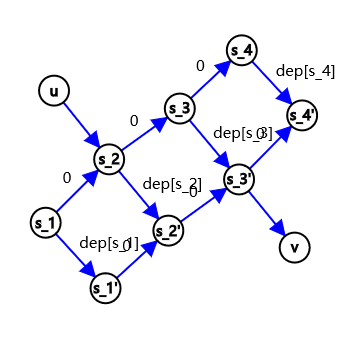
\includegraphics[width=3.0cm]{hacker.png}
			{\tiny \color{gray} 图有点丑,用CSAcademy上的graph\_editor随手画的}
		\end{center}
	
		上图解决了$x \le y$的情况,可以对称地解决另外一半。
		
	\end{block}
\end{frame}



\subsection{CERC2015 Juice Junctions}
\begin{frame}{CERC2015 Juice Junctions}
	\begin{block}{description}
		给出一张每个点度数不超过$3$的无向图,求两两节点之间的最小割(删去尽量少的边使得这两点不连通)。
	\end{block}
	\begin{block}{constraint}
		$n \le 3000, m \le 4500.$
	\end{block}
\end{frame}
\begin{frame}{CERC2015 Juice Junctions}
	\begin{block}{tutorial}
		显然最小割不超过$3$,那么就只会是$\{0, 1, 2, 3\}$中的某一个。	
		
		\begin{itemize}
			\item 当两个点连通时,它们的最小割$\ge 1$;
			\item 当两个点在同一个边双里时,它们的最小割$\ge 2$;
			\item 当两个点满足“删除任意一条边后仍在同一个边双里”时,它们的最小割$\ge 3$。
		\end{itemize}
	
		因此枚举每一条边删除后求边双即可。
	\end{block}
\end{frame}

\subsection{POI2013 Price List}
\begin{frame}{POI2013 Price List}
	\begin{block}{description}
		有一张$n$点$m$条边的无向图,每条边的边权都是$a$。
		
		现在对这张图进行一些操作:对于所有在原图中最短距离为$2a$的点对$(i, j)$,加入一条连接$i, j$且边权为$b$的边。
		
		求这张新图中指定源点$S$到其余每个点的最短路。
	\end{block}
	\begin{block}{constraint}
		$n, m \le 10^5.$
	\end{block}
\end{frame}
\begin{frame}{POI2013 Price List}
	\begin{block}{tutorial}
		可以发现新图上从$S$走到$T$的最短路的策略有且仅有如下三种:
		\begin{itemize}
			\item 只走$a$边,忽视加入的$b$边;
			\item 把两条$a$边并作一条$b$边走,最后视奇偶性可能会多出来一条$a$边;
			\item 只走$b$边。
		\end{itemize}
	
		前两种只需要对原图做一遍BFS。考虑第三种:当$u$点向外转移时,需要先枚举一个$u$的相邻点$v$,再枚举一个$v$的相邻点$w$,若$u, w$之间没有边,便可以从$u$来更新$w$。
		
		注意到这个过程中每个点只会被更新一次,所以一旦$u$成功更新$w$(等价于$u, w$之间没有边),$v \to w$这条枚举就可以删了。也就是说对于成功更新的部分,复杂度其实是关于一阶段枚举线性的,也即$O(m)$。
		
		问题在于不能成功更新的部分,即$u, w$之间有边,这会导致$(u, v, w)$构成一个三元环,而三元环个数是$O(m\sqrt m)$的,每个三元环对枚举复杂度的代价是常数的,因此总时间复杂度为$O(m\sqrt m)$。
	\end{block}
\end{frame}


\subsection{LOJ6078 重排}
\begin{frame}{LOJ6078 重排}
	\begin{block}{description}
		给你一张可能含重边自环的 DAG,边有边权。你要从 $s$ 走到 $t$。
		
		当你从一个点出发准备向外走时,这个点的所有出边的边权会被随机打乱。你可以知道打乱后每条边的边权分别是多少进而做出相应决策。
		
		求最短距离的期望。输出保留六位小数。
	\end{block}
	\begin{block}{constraint}
		$n, m \le 1000.$
	\end{block}
\end{frame}
\begin{frame}{LOJ6078 重排}
	\begin{block}{tutorial}
		先假设没有自环。按拓扑序逆序 dp,现在 $x$ 所有后继状态的 dp 值均已求出,我们想求要求 $dp_x$。\\
		
		假设 $x$ 的出边有 $k$ 条,后继状态有 $k$ 个,我们把这 $k \times k$ 个东西两两匹配,就得到了 $k^2$ 对二元组。将二元组按权值从小到大排序,依次考虑计算最终的最优方案大于等于当前二元组的权值的概率。算概率等同于算方案数,Rabbit Numbering(SRM 463) 即可。这样单
		点的复杂度就是 $O(k^2\log k)$,从 $m$ 分析上界就是 $O(m^2\log m)$。\\
		
		现在有自环了,因为只要求保留六位小数,所以可以二分求出 $dp_x$
		的近似解,具体来说就是每次把已有的 $dp_x$ 当做是一个后继状态
		并套用上面的做法,根据得到的新 $dp'_x$ 与 $dp_x$ 的大小关系来调整 $dp_x$ 的解。如果在加入自环的那些二元组时
		使用归并(将两个有序数组合并,复杂度线性),则可以将复杂
		度做到 $O(m^2\log m)$。
	\end{block}
\end{frame}


\subsection{CodeForces1110F Nearest Leaf}
\begin{frame}{CodeForces1110F Nearest Leaf}
	\begin{block}{description}
		给出一棵树,树边有边权。有$q$次询问,每次询问给出$v, l, r$,询问dfs序标号在$[l, r]$内的所有叶子到$v$的最远距离。
	\end{block}
	\begin{block}{constraint}
		$n, q \le 5 \times 10^5.$
	\end{block}
\end{frame}
\begin{frame}{CodeForces1110F Nearest Leaf}
	\begin{block}{tutorial}
		离线询问,先通过一遍DFS求出每个叶子到根的距离,再逐步移动询问点,每移动过一条边时,会导致一棵子树内的所有叶子的距离减去边权,而其他叶子的距离加上边权,用线段树维护即可。
	\end{block}
\end{frame}

\subsection{ARC087F Squirrel Migration}
\begin{frame}{ARC087F Squirrel Migration}
	\begin{block}{description}
		有一棵$n$个点的树。记$dis(i, j)$表示树上$i, j$两个点之间的距离,你需要生成一个排列$\{p_i\}$,最大化$$\sum_{i=1}^ndis(i, p_i)$$
		
		你需要求出这个最大化的结果,以及有多少个排列能使得上式取到最大值。
	\end{block}
	\begin{block}{constraint}
		$n \le 5000.$
	\end{block}
\end{frame}
\begin{frame}{ARC087F Squirrel Migration}
	\begin{block}{tutorial}
		(计数题乱入)\\
		
		对于一条树边$e$,假设其两边的子树大小分别是$sz_e$和$n - sz_e$,那么这条边对答案的贡献最多是$2\min\{sz_e, n - sz_e\}$。我们证明答案可以取到$2\sum_{e \in E}\min\{sz_e, n - sz_e\}$:只要选取一个点作为根,然后要求对于任意$i$,$i$与$p_i$均来自根的不同子树就可以了。显然我们会选择重心为根,并且一定能构造出一个满足条件的排列。\\
		
		对于有两个重心的情况,会发现只要让每个$i$匹配任意一个另一侧的点即可,因此方案数是$(\frac n2 !)^2$。\\
		
		对于有一个重心的情况,可以考虑容斥计算方案数(类似错排)。对于根的每一棵子树$u$,枚举其中有$0 \le k_u \le sz_u$个$i$强制匹配子树内的点,其余点随意匹配,对总方案数的贡献是$(-1)^{\sum k_u}(n-\sum k_u)!\prod \binom{sz_u}{k_u}^2k_u!$,DP计算即可。
	\end{block}
\end{frame}

\subsection{CSP-S2019 树的重心}
\begin{frame}{CSP-S2019 树的重心}
	\begin{block}{description}
		给出一棵树,对于一条树边$e$,记$S_e$表示把$e$从树上删去后,剩下的两棵树上的重心的标号之和。求$\sum_{e \in E}S_e$。
	\end{block}
	\begin{block}{constraint}
		$n \le 3 \times 10^5.$
	\end{block}
\end{frame}
\begin{frame}{CSP-S2019 树的重心}
	\begin{block}{tutorial}
		固定一个点$x$,统计割掉哪些边后,可以使$x$称为重心。\\
		
		取原树的某个重心$r$作为根。当$x \neq r$时,那么割掉的边必然要在子树外,且被割掉的部分会受到一个大小限制,可以用树状数组来统计。“在子树外”的条件可以用全集减去在子树内的,可以通过一些技巧实现“在子树内”这一限制。\\
		
		当$x = r$时,需要考虑割掉的边是否来自最大的子树,会分别得到不同的大小限制,同样用树状数组简单统计即可。
	\end{block}
\end{frame}

\subsection{CEOI2019 动态直径}
\begin{frame}{CEOI2019 动态直径}
	\begin{block}{description}
		一棵$n$个点的树,每条边都有一个非负边权。
		
		有$q$次修改操作,每次修改一条边的权值,并询问树的直径。
	\end{block}
	\begin{block}{constraint}
		$n, q \le 10^5.$
	\end{block}
\end{frame}
\begin{frame}{CEOI2019 动态直径}
	\begin{block}{tutorial}
		线段树维护直径即可。合并即利用直径合并的结论。
	\end{block}
\end{frame}
\subsection{ZJOI2019 语言}
\begin{frame}{ZJOI2019 语言}
	\begin{block}{description}
		给一棵$n$个点的树和树上的$m$条路径,问有多少对$(i,j)$满足这两点同时被至少一条路径覆盖。
	\end{block}
	\begin{block}{constriction}
		$1 \le n, m \le 10^5.$
	\end{block}
\end{frame}
\begin{frame}{ZJOI2019 语言}
	\begin{block}{tutorial}
		对每个点求所有覆盖该点的链的链并大小,加起来除以$2$就是答案。
		
		树上差分,即对于链$(x,y)$在$x$和$y$处加入这两个点,在$fa_{lca(x,y)}$处删去(注意判出现次数)。线段树合并即可,复杂度$O(n\log n)$。
		
	\end{block}
\end{frame}

\subsection{POI2014 Hotel}
\begin{frame}{POI2014 Hotel}
	\begin{block}{description}
		给一棵$n$个点的树,从中选$3$个点使两两距离相同,求方案数。
	\end{block}
	\begin{block}{constraint}
		原问题$n \le 5000$,加强版$n \le 10^6.$
	\end{block}
\end{frame}
\begin{frame}{POI2014 Hotel}
	\begin{block}{tutorial}
		考虑朴素做法。记$f_{i,j}$表示节点$i$子树内和$i$的距离为$j$的点数,$g_{i,j}$表示节点$i$子树内满足第三个点(在子树外)和$i$的距离为$j$的点对数目。\\
		
		这样每次可以拿$f_{u,j}\times g_{v,j+1}$和$g_{u,j+1}\times f_{v,j}$更新答案,拿$f_{u,j}\times f_{v,j-1}$更新$g_{u,j}$,$f_{v,j}$更新$f_{u,j+1}$,$g_{v,j}$更新$g_{u,j-1}$,其中$v$是$u$的一个轻儿子。\\
		
		仔细观察会发现,$g$数组的更新与$f$是相反的,所以$g$数组反着开就行了。
		
	\end{block}
\end{frame}

\subsection{Wannafly挑战赛12F 小H和圣诞树}
\begin{frame}{Wannafly挑战赛12F 小H和圣诞树}
\begin{block}{description}
	一棵$n$个点的树,每个点有个颜色$col_i$,每条边有个边权。
	
	$q$次询问,每次给两种颜色$a,b$,求$\sum_{col_x=a,col_y=b}dist(x,y)$。
\end{block}
\begin{block}{constriction}
	$1 \le n, m \le 10^5.$
\end{block}
\end{frame}
\begin{frame}{Wannafly挑战赛12F 小H和圣诞树}
\begin{block}{tutorial}
	设置阈值$S$。\\
	
	对于一种出现次数超过$S$的颜色,做两遍DFS对每个点预处理出“到所有该颜色点的距离和”。\\
	
	查询时若一种颜色的出现次数超过$S$,则直接暴力枚举较少的一种颜色统计答案;否则两种颜色的出现次数都不超过$S$,把这不超过$2S$个点拿出来建虚树后做前述的两遍DFS(最好对多组涉及同一种颜色的询问一起做)。\\
	
	总时间复杂度为$O(\frac{n^2}{S}+n\sqrt n+nS\log n)$,当$S$取$O(\sqrt{\frac{n}{\log n}})$时,复杂度为$O(n\sqrt{n\log n})$。(默认$n,q$同阶)
\end{block}
\end{frame}


\section{The end}
\begin{frame}
	\begin{center}
		{\huge 谢谢大家!\\  \large 祝大家学业有成!}
	\end{center}
\end{frame}

\end{document}